\documentclass[fleqn,10pt]{olplainarticle}
\usepackage{float}
\usepackage{tikz}
\usepackage{caption}
\usepackage{subcaption}
\usepackage{hyperref}
\hypersetup{
    colorlinks=false,
    pdfborder={0 0 0},
}
\usepackage{pgfplotstable,filecontents}

% Use option lineno for line numbers
%\title{What is the cause and effect in ship data analysis, when all we can see is correlation?}
\title{Causal inference for fuel consumption optimization of a double ended ferry}



\author[1,2]{Martin Alexandersson}
\affil[1]{Research Institutes of Sweden (RISE), Chalmers tvärgata 10, 41296 Gothenburg Sweden}
\affil[2]{Dept. of Mechanics and Maritime Sciences, Division of Marine Technology,
                                Chalmers University of Technology, Hörsalsvägen 7A, Gothenburg Sweden}

\keywords{Ship dynamics, Causal inference, System identification, Monte Carlo simulations, Markov chain analysis}



\begin{abstract}
\setlength{\parindent}{10pt}
% Move 1 - Background/introduction/situation
Statistical analysis or machine learning (ML) on real data can be used to propose changes in optimizing a system's behaviour. Before such changes could be proposed, determining the cause and effect relation between the variables -- causality -- is necessary.
The aim of standard statistical analysis or ML is to find trends or associations between variables. 
For these trends to be usable in optimization, we need to move one step further, also trying to find the causality.

% Move 2 - Present research/purpose
In this paper, causal inference is investigated on a dataset collected onboard the double ended ferry Uraniborg.
A previously observed trend with high correlation between thruster utilization (TU) and fuel consumption (FC) is investigated to see if there is direct causality, which can then be used to optimize the FC.

% Move 3 - Methods/materials/subjects/procedures
The inference was conducted with a controlled experiment onboard the ship, where the operation of the ship was altered between the captain and mate, every other journey.
% Move 4 - Results/findings
The experiment showed that there is most likely a direct causal relationship between the TU and FC.
An optimized TU, where only the aft thruster is utilized, is estimated to have between 9 and 17\% lower FC compared to the previous operation of the ship.

% Move 5 - Discussion/conclusion/significance
The experiment showed that it is possible to conduct a reasonably controlled experiment onboard a real ship during operation to infer the causality between the TU and FC.
This technique can be used within ship operational data analysis, where an associative analysis obtained with ML -- as correlations or regressions --  can be accompanied with a causal analysis, so that the identified association can be used to optimize the ship's operation.







\end{abstract}
\newcommand\savingpctexperiment{17}
\begin{document}
\def\equationautorefname~#1\null{Eq.~(#1)\null}
\def\figureautorefname~#1\null{Figure~#1\null}
\def\tableautorefname~#1\null{Table~#1\null}

\flushbottom
\maketitle
\thispagestyle{empty}
\newpage
\section{Introduction}
%________________________________________
%CaRS Move I "Establish a territory" (Situation):
% * Important area
% * Introducing and reviewing items of previous  research <--(ToDO)

As humans, we often think in terms of cause and effect -- causality; if we understand why something happened, we can change our behavior to improve future outcomes. 
Causal inference is a process of determining the causality. The inference can be conducted in a controlled experiments, where the effect of one variable can be studied in isolation.
Some problems are however unsuitable for controlled experiments, where causal inference thus becomes more difficult. Determining the causality from real world data is such a problem, which can be difficult yet very important; for instance: to convincingly show that the emission of green house gases causes global warming, is perhaps the most important problem of our time? 

Data analysis can be used to show how variables vary together (correlation); however, correlation does not imply direct causality where: \emph{A} causes \emph{B} (\autoref{fig:direct_causation}). It could also be the opposite relation -- reversed causality (\autoref{fig:reversed_causation}). 
For instance: \emph{do windmills generate the wind, or is it the other way around?} There could also be a third hidden variable \emph{C}, causing both \emph{A} and \emph{B} -- common causality (\autoref{fig:common_causation}). For instance: \emph{if ice cream sales increase, the rate of drowning deaths also increases, so should you avoid ice cream when swimming?}
\begin{figure}[!htb]
    \begin{subfigure}[b]{0.3\textwidth}
        \centering
        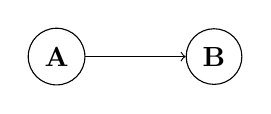
\begin{tikzpicture}[node distance=2cm]
        \node[circle,draw] at (0,0) (A) {\bf A};
        \node[circle,draw,right of=A] (B) {\bf B};
        \draw[->] (A) -- (B);
        \end{tikzpicture}
        \caption{Direct causality}
        \label{fig:direct_causation}
    \end{subfigure}
    \hfill
    \begin{subfigure}[b]{0.3\textwidth}
        \centering
        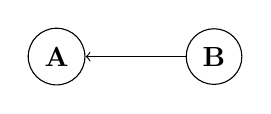
\begin{tikzpicture}[node distance=2cm]
        \node[circle,draw] at (0,0) (A) {\bf A};
        \node[circle,draw,right of=A] (B) {\bf B};
        \draw[<-] (A) -- (B);
        \end{tikzpicture}
        \caption{Reversed causality}
        \label{fig:reversed_causation}
    \end{subfigure}
    \hfill
    \begin{subfigure}[b]{0.3\textwidth}
        \centering
        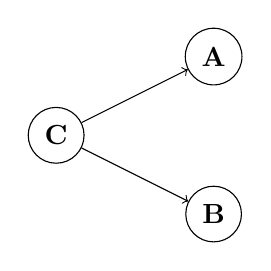
\begin{tikzpicture}[node distance=2cm]
        \node[circle,draw] at (0,0) (C) {\bf C};
        \node[circle,draw,right of=C,yshift=1cm] (A) {\bf A};
        \node[circle,draw,right of=C,yshift=-1cm] (B) {\bf B};
        \draw[->] (C) -- (A);
        \draw[->] (C) -- (B);
        \end{tikzpicture}
        \caption{Common causality}
        \label{fig:common_causation}
    \end{subfigure}
    \caption{Causality}
    \label{fig:causal_relationships}
    
\end{figure}

In ship hydrodynamics, experiments in a controlled laboratory environment with scale models (model tests) is a well established causal inference method.  
The model tests have some drawbacks such as: scale effects, and the fact that the laboratory environment as well as the test scenario are artificial idealizations of their real counterparts.
Data driven analysis on real ship operational data, instead of model tests, is a more direct way to analyze the ship's hydrodynamics, which has become more popular during the last years. The increased data collection onboard ships, as well as advancements within machine learning (ML), are probable drivers in this development. 

%________________________________________
%CaRS Move II "Establish a niche" (Problem):
% * counter claim?
% * gap?
% * question       <------
% * continuation? 
However, the real ship operational data is usually not collected from a controlled experiment, so that the causal inference thus becomes more challenging. Such a challenge is addressed in this paper: investigating a possible causal relationship between thrust allocation and fuel consumption of a double ended ferry -- Uraniborg (\autoref{fig:uraniborg}).
\begin{figure}[!htb]
    \centering
    \includegraphics[width=0.7\textwidth]{figures/GA_uraniborg.pdf}
    \caption{Double ended ferry Uraniborg, copyright Rederi AB Ventrafiken.}
    \label{fig:uraniborg}
\end{figure}
The thrust allocation concerns the load balance between the the ship's two azimuth thrusters: one in the aft, and one in the bow of the ship (\autoref{fig:uraniborg}). The two thrusters can run simultaneously, adding up to the total thrust force, driving the ship forward. The load balance can vary between all combinations from: full aft, to full forward thruster utilization (TU). This balance can be expressed with \autoref{eq:aft_thrust_ratio},
\begin{equation}
    TU = \frac{C_{aft}}{C_{aft} + C_{fwd}}
    \label{eq:aft_thrust_ratio}
\end{equation}
where $C_{aft}$ and $C_{fwd}$ are the fuel consumption from the aft and forward thruster.
\autoref{fig:fuel_consumption_correlation} shows data from trips between Landskrona and Ven during one year for the variables: total fuel consumption, and $TU$. There seems to be a clear correlation between these variables,  which implies that there is relationship between them. But is it a direct causal relationship? Direct causality would mean that $TU$ can be used as an optimization parameter to reduce the fuel consumption.
\begin{figure}[!htb]
    \centering
    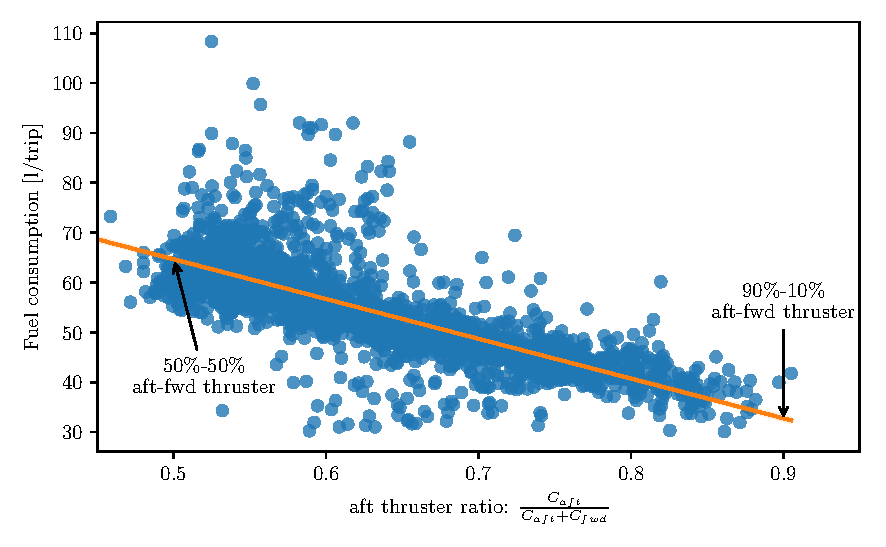
\includegraphics[width=\textwidth]{figures/correlation.pdf}
    \caption{Fuel consumption per trip with Uraniborg for trips during one year with varying aft thrust ratio.}
    \label{fig:fuel_consumption_correlation}
\end{figure}
However, both reversed causality or common causality are other possibilities, considering for instance these hypothetical scenarios:
\begin{itemize}
    \item Increased fuel consumption forces a reduced aft thruster utilization if the aft thruster is not strong enough. The forward thruster is then needed to add up to the higher power demand. (Reversed causality)

    \item There is a hidden variable such as bad weather which forces both thrusters to be used. (Common causality)
\end{itemize}
%________________________________________

%CaRS Move III "Occupy the niche" (Solution/Evaluation):
% * outline purpose?
% * list research questions?
% * announce principal findings?            <--
% * stating the value of present research?
% * article structure?                      <--
A controlled experiment was conducted onboard Uraniborg to infer the direct causal relationship. Results from this experiment are presented and analyzed in this paper to conclude the relationship. Alternative methods applicable when experiments are not possible, are also discussed and investigated. Conducting system identification on a well established physical model is one of these methods, which is presented in this paper. Also Monte Carlo simulations, and Markov chain analysis are alternatives that are discussed, but more briefly. To complete this paper, it is investigated if the alternative methods can reach to the same conclusion as obtained from the controlled experiment inference.

\section{Method}
A controlled experiment (\autoref{sec:blinded_experiment}) is the classic way to determine the causation. System identification with well established mathematical models, Monte Carlo simulations, and Markov chain analysis are alternatives that can be used for situations where experiments cannot be conducted

\subsection{Controlled experiment}\label{sec:blinded_experiment}
In the controlled experiment, every other trip with Uraniborg was run with two different crews. One crew was operating as normal and the other crew was instructed to only use the aft thruster as much as possible. The same correlation that was seen in \autoref{fig:fuel_consumption_correlation} was observed again during the experiment and a direct causation was concluded that a higher use of the aft thruster will reduce the fuel consumption.

\subsection{System identification}
\subsection{Monte Carlo simulations}
\subsection{Markov chain analysis}
\section{Results and discussion}
The fuel consumption of Uraniborg with the speed correction applied, is shown in \autoref{tab:means_corrected} for the four datasets: ship operation by the captain and mate during experiment and the reference period. The captain had much lower fuel consumption compared to the mate for both periods. Even though the captain used a little bit higher aft thruster utilization already before the experiment (0.8 compared to 0.7), there can also be other explanations to the captains's lower consumption such as: higher skills and experience in operating the ship.
The difference was however much larger during the experiment (\savingpctexperiment \%), compared to the reference period (\savingpctbeforeexperiment \%). The captain used a lower aft thruster utilization (TU=0.8) before the experiment compared to during the experiment, where aft thruster was used exclusively (TU=1). This means that at least \savingthrusterallocationpct \% of the total \savingpctexperiment \% reduction can be accounted to the increased aft thruster utilization.
The remaining difference between the fuel consumption of the captain and mate during the experiment (\savingpctbeforeexperiment \%) needs futher investigations. It would be a good idea to get a closer look at how the captain and mate operate the ship, to find an explanation how to operate the ship in the more energy efficient way of the captain.

\begin{table}[h]
    \centering
    \caption{Mean values corrected for differences in speeds in the original data for the four datasets where the ship is operated by the captain or mate during the reference period or experiment. The number of trips is also shown for each period.}
    \label{tab:means_corrected}
    \pgfplotstabletypeset[col sep=comma,
    columns={Operator,Period, sog, TU,Consumption,Trips},
    columns/Operator/.style={string type},
    columns/Period/.style={string type},
    column type=l,	% specify the align method
	every head row/.style={before row=\hline,after row=\hline},	% style the first row
	every last row/.style={after row=\hline},	% style the last row
	%every first column/.style={column type/.add={|}{}},	% style the first column
	%every last column/.style={column type/.add={}{|}},	% style the last column
    ]{tables/tab_means_corrected.csv}
\end{table}

\section{Conclusions}
%_________________________________________________________
%Move 1: Background information (research purposes, theory,
%methodology)
A high correlation between the aft thruster utilization (TU) and fuel consumption (FC) has previously been observed for trips between Landskrona and Ven with the double ended ferry Uraniborg.  A controlled experiment was conducted onboard the ship, where the TU was varied to infer if the observed correlation implies a direct causal relationship. Such a relationship would mean that the TU can be used as an optimization parameter for FC reduction.

The experiment was conducted with two different operators of the ship: the captain and the first mate. The captain was instructed to operate the ship in a new way: with as much aft thruster utilization as possible; the first mate was instructed to run the ship in a more normal way: using both the forward and aft thruster.
To obtain a reliable inference, the TU needs to be the only parameter varied during the experiment. A procedure where the operator was changed every other round trip, was therefore adopted. Ideally, the operators would face as similar conditions as possible, in terms of traffic, wind, waves, and currents.
Differences in ship speed during the experiments where therefore also corrected with a FC prediction model.

%_________________________________________________________
%Move 2: Summarizing and reporting key results. (oblig.)
The experiment was conducted according to the plan where the captain used the aft thruster almost exclusively, obtaining an average TU of 0.99, while during the same time, the mate used a more normal operation (TU=0.69). The difference in FC during the experiment, between the two operators, was substantial: with \savingpctexperiment \% lower FC for the captain. 
%_________________________________________________________
%Move 3: Commenting on key results (making claims, explaining the results,
%comparing the new work with previous studies, offering
%alternative explanations) (oblig.)
The experimental results were also compared with data collected from a reference period before the experiment, with the same operators running the ship on a similar schedule. The captain had a much lower average (TU=0.77) during the reference period compared to the experiment, in contrast to the mate who had a similar TU for both periods. The captain had a lower FC during the reference period as well (\savingpctbeforeexperiment \%).
The reduction was however much larger during the experiment, which most likely implies that there is a direct causality between TU and FC; the increased TU, used by the captain during the experiment, seems to have caused a substantial reduction of the FC. The FC reduction from increased TU (0.77 to 0.99) is estimated to be at least \savingthrusterallocationpct \%, when subtracting the reference period reduction -- between captain and mate -- from the FC reduction obtained at the experiment. 
% previous studies: "designing a double ended ferry"

%_________________________________________________________
%Move 4: Stating the limitations of the study
The experiment was conducted during three days of relatively good weather with two operators that run the ship quite differently, already from before the experiment.
A repeated experiment, during other weather conditions, and with other operators --   who preferably have a more similar operation -- would increase the confidence in the present results.

%_________________________________________________________
%Move 5: Making recommendations for future implementation and/or for
%future research
The captains reduced FC before the experiment, can partly be explained by a higher TU  than the mate. % Is this the whole explanation?
This reduction is however still partly unexplained and requires more thorough investigations that could lead to suggestions for further FC reductions of Uraniborg.

\bibliography{sample}

\end{document} 